\section{Lựa chọn Dataset và Xây dựng Mô hình Dữ liệu}
\label{sec:data_model}

Chương này dùng để mô tả chi tiết về nguồn gốc bộ dữ liệu, cấu trúc các bảng dữ liệu quan hệ, quy trình tiền xử lý dữ liệu và cách thiết lập mô hình dữ liệu trong Power BI của nhóm.

\subsection{Giới thiệu nguồn dữ liệu và lý do lựa chọn}
\textit{[Hướng dẫn điền: Nhóm tự điền thông tin giới thiệu nguồn dữ liệu mà nhóm đã thống nhất lựa chọn (ví dụ: Kaggle, World Bank, Data.gov...). Nêu rõ lý do lựa chọn bộ dữ liệu này (kích thước dữ liệu, tính thực tiễn, mức độ phong phú của các mối quan hệ giữa các bảng) và cung cấp đường dẫn/liên kết tải dữ liệu công khai].}

\subsection{Mô tả các bảng dữ liệu và trường thông tin quan trọng}
Bộ dữ liệu sử dụng trong đồ án là cơ sở dữ liệu quan hệ (relational dataset) gồm ít nhất 2-3 bảng dữ liệu có liên kết với nhau. Dưới đây là mô tả chi tiết cấu trúc các bảng dữ liệu của nhóm:

\begin{enumerate}
    \item \textbf{Bảng dữ liệu chính (Fact Table - Ví dụ: Bảng giao dịch, bảng sự kiện...)}:
    \begin{itemize}
        \item \texttt{[Tên trường khóa chính]} (Khóa chính): Mã định danh duy nhất của mỗi dòng giao dịch.
        \item \texttt{[Tên trường khóa ngoại]} (Khóa ngoại): Liên kết đến các bảng chiều (Dimension tables).
        \item \texttt{[Tên trường số đo lường]} (Ví dụ: Doanh số, số lượng, điểm số, thời gian...): Các biến định lượng dùng để tính toán chỉ số.
        \item \texttt{[Mô tả các trường thông tin khác...]}
    \end{itemize}
    
    \item \textbf{Bảng dữ liệu chiều thứ nhất (Dimension Table 1 - Ví dụ: Khách hàng, sản phẩm, địa điểm...)}:
    \begin{itemize}
        \item \texttt{[Tên trường khóa chính]} (Khóa chính): Mã định danh duy nhất của thực thể.
        \item \texttt{[Các trường thuộc tính]} (Ví dụ: Tên, phân loại, trạng thái...): Dùng để lọc và phân nhóm dữ liệu.
    \end{itemize}

    \item \textbf{Bảng dữ liệu chiều thứ hai (Dimension Table 2 - Ví dụ: Thời gian, chi nhánh, loại hình...)}:
    \begin{itemize}
        \item \texttt{[Tên trường khóa chính]} (Khóa chính): Mã định danh duy nhất của thực thể.
        \item \texttt{[Các trường thuộc tính]} (Ví dụ: Địa chỉ, vùng miền, danh mục con...): Dùng để lọc và phân nhóm dữ liệu.
    \end{itemize}
    
    \item \textit{[Thêm các bảng khác nếu có...]}
\end{enumerate}

\subsection{Mô hình dữ liệu quan hệ (Data Model) trong Power BI}
Sau khi nạp các bảng dữ liệu vào Power BI Desktop, nhóm tiến hành thiết lập mối quan hệ giữa các bảng (quan hệ một - nhiều $1:\infty$ hoặc một - một $1:1$ thông qua các trường khóa ngoại) để tạo thành mô hình hình sao (Star Schema) hoặc mô hình bông tuyết (Snowflake Schema):

\begin{figure}[H]
    \centering
    % Nhóm sẽ chụp ảnh màn hình Model View thực tế trong Power BI của mình và lưu đè lên file này
    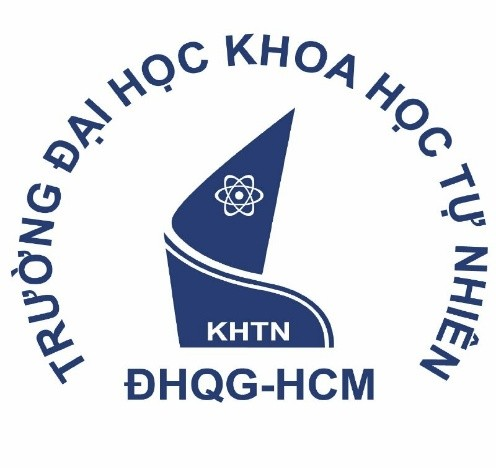
\includegraphics[width=0.85\textwidth, keepaspectratio]{images/data_model_diagram.png}
    \caption{Sơ đồ mối quan hệ (Data Model) thực tế trong Power BI của nhóm}
    \label{fig:data_model}
\end{figure}

\textit{[Nhóm tự điền: Mô tả chi tiết mối quan hệ giữa các bảng đã liên kết. Ví dụ: Bảng A liên kết với bảng B qua trường khóa X với kiểu liên kết một-nhiều và chiều lọc hướng từ A sang B].}

\subsection{Quy trình tiền xử lý dữ liệu (Power Query)}
Dữ liệu thô khi tải về thường chưa sẵn sàng để phân tích ngay, nhóm đã thực hiện quy trình làm sạch và tiền xử lý dữ liệu qua các bước sau trên Power Query Editor:
\begin{enumerate}
    \item \textbf{Xử lý giá trị trống hoặc lỗi (Null/Missing/Error Values)}: \textit{[Mô tả cách xử lý của nhóm, ví dụ: xóa dòng lỗi, điền giá trị trung vị hoặc giá trị mặc định cho ô trống...]}.
    \item \textbf{Chuẩn hóa kiểu dữ liệu (Data Type Correction)}: \textit{[Mô tả cách chuẩn hóa định dạng số, ngày tháng, văn bản để tránh lỗi tính toán và lỗi phân tích địa lý...]}.
    \item \textbf{Biến đổi và trích xuất đặc trưng (Feature Engineering)}: \textit{[Mô tả việc tách/gộp cột, tạo cột mới từ cột cũ, tạo bảng Calendar (bảng Date) bằng DAX hoặc Power Query để hỗ trợ phân tích thời gian...]}.
    \item \textbf{Nối hoặc Gộp các bảng (Append/Merge Queries - Nếu có)}: \textit{[Mô tả cách gộp các file lẻ thành bảng lớn nếu có...]}.
\end{enumerate}
Quá trình tiền xử lý này đảm bảo dữ liệu luôn nhất quán, chính xác, giúp tối ưu hóa hiệu năng tính toán các measure DAX trong Power BI.
